\chapter{Experimental results \status{in progress}}
\label{chap:results}

In this chapter we quantitatively and qualitatively analyse the performance of the automatic cell detector and tracker. Although some evaluation of the performance of the detection method is performed by the original authors in \cite{arteta12} it is useful to see how the method performs on the studied datasets in order to understand how much of the tracking accuracy is lost due to cells missed by the detection module. First, in \cref{sec:results_detector} we evaluate the performance and computation time of the cell detector and in \cref{sec:results_tracker} those of the cell tracker. Finally, in \cref{sec:results_limitations}, we explore the limitations of the methods and in \cref{sec:results_summary} summarize the results.

\todo[inline]{See the cell population tracking and linear construction with spationtemporal ocntet by Kang et al for a good results section}

\section{Cell detector \status{in progress}}
	\label{sec:results_detector}
	
	In this section we evaluated the performance of the automatic cell detection module. First, we introduce the performance metrics used to evaluate the accuracy of the cell detector. Then we present detection accuracy results. To evaluate the accuracy and generalizability of the detection module we perform two sets of experiments. First, we train the cell detector on a number of frames from each individual dataset, and measure the accuracy on the same dataset. Second, we train the detector on combinations of datasets in order to judge the performance degradation due to the learning on the more types of cells. Because of the varying size of the cells in the datasets, and the varying brightness of the cells, we expect that such a trained detector will perform poorer than when trained and tested on individual datasets, sometimes mistakenly detecting small artefacts in the background as cells. Finally, we compute the average detection time per frame for each dataset.
	
	The aim of this research was to develop an automatic cell detection and tracking pipeline that would require as little manual work as possible. This implies that a balance between accuracy and amount of manual work had to be established. There is also an direct relationship between accuracy and computation time. In order to reduce the amount of manual work we aimed to configure the cell detection module such that it would perform well on all the tested datasets without any manual adjustments of parameters. The consequences of this decision are twofold:
	
	\begin{enumerate}
		\item The features computed on the candidate cell regions are the same for all datasets and have been presented in \cref{sec:detector_feature}. Although some datasets could be analysed faster or more accurately with a different subset of features, using the same features for all dataset eliminates the complicated feature selection process for the user and makes the system generalizable to a large number of different cell types.
		
		\item The parameters of the MSER detector should be adequately set to perform well on all datasets. This means that the MSER detector should be able to detect cells of varying size and contrast in the different datasets. The consequence of this limitation for datasets with large cells and some background noise is that a potentially much larger number of candidate regions will be detected than necessary. Since each candidate region has to be evaluated this results in an increased computation time.
	\end{enumerate}
	
	We were able to identify features that compute in an acceptable time for all these datasets (see \cref{sec:detector_feature}). However, it should be noted that in the case of testing the detector on very large datasets with thousands of frames, some adjustments of the parameters could result in a significant reduction in computation time and increased accuracy.
	
	\subsection{Performance metrics \statusnew}
	
	We measure the performance of the cell detector in terms of precision and recall. The metrics are defined in terms of:
	
	\begin{description}
		\item[True Positive instances] (TP) are candidate cell regions that are manually annotated as cells and the detector successfully classified as cells.
		\item[False Positive instances] (FP) are candidate cell regions that are not manually annotated as cells, but the detector incorrectly classified them as cells.
		\item[False Negative instances] (FN) are candidate cell regions that are manually annotated as cells, but the detector incorrectly classified.
	\end{description}
	
	We then define precision as:
	
	\[
		\text{PRE} = \frac{\text{TP}}{\text{TP}+\text{FP}}\text{,}
	\]
	
	\noindent and recall (also known as sensitivity) as:
	
	\[
		\text{REC} = \frac{\text{TP}}{\text{TP} + \text{FN}}\ \text{.}
	\]
	
	\subsection{Detection accuracy \statusnew}
			
		As mentioned previously, we performed two different experiments to measure the performance of the cell detection module. The first experiment consisted of training and testing of the algorithm on the same dataset. The training set was 70\% and the testing set 30\% of the entire dataset. The training and testing datasets were created from images in randomized order from the entire dataset. This allowed us to measure, for each dataset, the maximum precision and recall values we could expect from the algorithm. In the second experiment the training was performed on combined datasets. The goal of this experiment was to observe how well the algorithm is able to generalize, and still return acceptable results.
		
		\subsubsection{Training and testing on single dataset}
		
		The training was performed on 70\% of the manually dot-annotated images from each dataset, and tested on the remaining 30\%. \Cref{tab:results_detector_individual} displays the computed precision and recall values, together with the total number of cells that were annotated in each dataset.
		
		\todo{Repeat the measurements with the best feature selection}
		
		\begin{table}[h]
			\centering
			\begin{tabular}{rrr}
				Dataset & Precision $\left[ \% \right]$ & Recall $\left[ \% \right]$ \\
			\hline
				      A &                          58.3 &                       45.4 \\
				      B &                          89.8 &                       93.6 \\
				      C &                          82.5 &                       81.6 \\
				      D &                          81.9 &                       90.5 \\
				      E &                          82.3 &                       94.9
			\end{tabular} 
			\caption{Precision and recall values for the cell detector trained on each dataset individually.}
			\label{tab:results_detector_individual}
		\end{table}
		
		\todo{Explain why detection can be bad on dataset A}
		   	% THE problem with this dataset is the sudden change of contrast when it
		   	        % switches from frame 17 to 18. At that point all the background starts
		   	        % looking like all the positive examples in the previous frames, which means
		   	        % that a lot of negative examples are generated which cancel out all
		   	        % learned in the first 17 frames

		\todo{Discuss: which better, why(better images? less noise?), what could be improved...}
		
		\subsubsection{Training on composite dataset}
		
		In this second experiment we were instered in measuring how well the algorithm is able to generalize when it is trained on a larger, combined dataset. For this purpose, several of the datasets were grouped, and the detector was trained to recognize cells of all types. Then, the results were tested individually on the 30\% of the annotated images from each dataset, that were not used for training. \Cref{tab:results_detector_combined} shows the results.
		
		
		\todo{Repeat the measurements with the best feature selection}
		
		\todo{Try different dataset combinations based on the observations... similar datasets}
		
		\begin{table}[h]
			\centering
			\begin{tabular}{rrrr}
				Combined dataset &                  Precision $\left[ \% \right]$ &                     Recall $\left[ \% \right]$ &  \\
			\hline
				       A+B+C+D+E & A: 60, B: 60, C: 60, D: 60, E: 60 & A: 60, B: 60, C: 60, D: 60, E: 60 &
			\end{tabular} 
			\caption{Precision and recall values for the cell detector trained on combined datasets.}
			\label{tab:results_detector_combined}
		\end{table}
				
		\todo{Add discussion: generally how much precision/recall we loose, which dataset seems to suffer less/more, why do they suffer less/more (have fewer cells to be trained on, like like noise in another dataset)}
		
		
		\todo{Here show an example of detection in a dataset so the use has a better idea of the difficulty of connecting the dots, like this image below...maybe create one for each dataset}
		Figure \ref{fig:results_cell_tracks_detection} displays a temporal view of the detected cells. The vertical axis represents the frame of the sequence. The figure clearly shows that ``cell tracks'' are clearly discernible, even if the number of outliers is significant. For the tracking module it is better to have a higher recall than precision, as outliers can be much more easily discarded than segmented tracks linked.
		\begin{figure}
			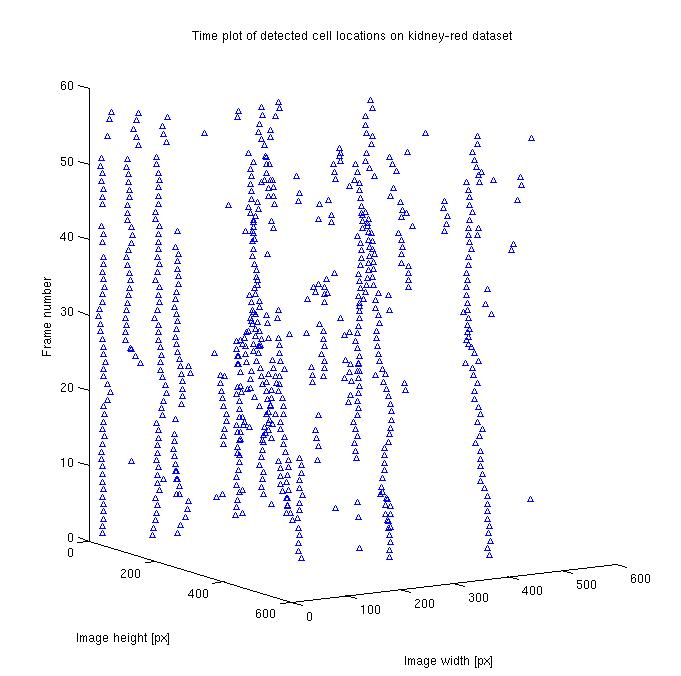
\includegraphics[width=\textwidth]{images/cell_tracks}
				\caption{Cells detected over 60 consecutive frames are visualized as a time series. The vertical axis corresponds to the frames. Even in this raw detection data, it is possible to see the tracks of some of these cells.}
			\label{fig:results_cell_tracks_detection}
		\end{figure}
			
				
		
	\subsection{Computations time \statusnew}
	
		In order to positionally track cells in image sequence the computation time of extracting the cell position from each frame is just as important as the accurate identification of cells. \Cref{tab:results_detector_speed} displays the average detection times per frame for each dataset. The detection time is dependent on the number of candidate cell regions extracted and their dimensions.
		
		\todo{Explain hardware and software, say 1 core... can use more}
		
		\todo{It might be useful to show the comparison with the old detector if I have the time}
		
		\todo[inline]{Measure the speed of detection in images of different sizes, and different number of cells}
		
		\todo[inline]{Explain what the candidate-annoation ration is, and what it tells. Also the ocmputations timer per candidate vary from 0.0086-0.0226}
		
		\begin{table}[h]
			\centering
			\begin{tabular}{rrrr}
				Dataset & Time per frame  $\left[ s \right]$ & Time per annotated cell  $\left[ s \right]$ & Candidate-Annotation ratio \\
			\hline
				      A &                             0.9224 &                                      0.5854 &                       26:1 \\
				      B &                             1.5899 &                                      0.2015 &                       16:1 \\
				      C &                             1.1214 &                                      0.0586 &                        7:1 \\
				      D &                             1.5215 &                                      0.1454 &                       18:1 \\
				      E &                             0.6016 &                                      0.0853 &                        9:1
			\end{tabular} 
			\caption{Average computation times per frame and annotated cell using a single worker.}
			\label{tab:results_detector_speed}
		\end{table}
		
		\todo{Discuss which is faster, try to explain why-- less noise -- less candidate cells... }
	
\section{Cell tracker \statusnew}
	\label{sec:results_tracker}
	\todo[inline]{Define the different measures of accuracy}
	\subsection{Performance metrics \statusnew}
	
	TODO: test detector on full dataset, but train it on ALL (notjust70\%) of the annotation
	TODO: train tracker on 70\% of the trajectories, test on rest
	
	great Metrics: Research Article, Evaluating Multiple Object Tracking Performance: The CLEAR MOT Metrics
	
	- Explain how the testing data was generation. from annotation to mapped deteciton to genreated tracklets

	\subsection{Tracking accuracy \statusnew}
		- trained on single dataset
		
		- for each dataset explain how the parameters were setup
					
		- trained on combined dataset
	\subsection{Computation time \statusnew}
	\todo[inline]{Meause the speed of generating tracks, as a measure of per 1, 100, 1000 frames, depending on the number of tracks}
\section{Limitations and areas of improvement \statusnew}
	\label{sec:results_limitations}
	Answer: what, why, how to improve in future
			
	- display examples where the tracker did not perform well, and anlyse why. Suggest possible improvement.
	- detection training: only first few frames of datasets, not random -- expect to detect later frames worse
	- testing on only long datasets: no data on short datasets. diffucult to train (what to link?), difficult to annotate
	- speed of detector. Reduce number of hypothesis		

\section{Summary \statusnew}
	\label{sec:results_summary}
	Brief review of accuracy... whether it is comparable to other methods in literuature review
	Whether is could be improved in the future... how much